\documentclass[10pt,a4paper]{scrartcl}
% scrartcl.cls, scrreprt.cls, scrbook.cls ??? created from european point of view
% KOMA-script package required for these layouts

\usepackage[top=2.5cm, bottom=3cm, left=2cm, right=2cm]{geometry}

\usepackage[pdftex]{graphicx}
\usepackage[english]{babel}
\usepackage{palatino}
\usepackage{relsize}
\usepackage{multicol}
\usepackage{blindtext}
\usepackage{setspace}
\usepackage[absolute]{textpos} % places boxes at an absolute position - used for placing the logo's on the cover page
    \setlength{\TPHorizModule}{1mm}            % length of 1 unit horizontally
    \setlength{\TPVertModule}{\TPHorizModule}   % length of 1 unit vertically
    \textblockorigin{0mm}{0mm} % position from the top left from where positions are calculated
    \setlength{\parindent}{0pt}
%\usepackage{a4wide}                     % Iets meer tekst op een bladzijde
% the a4wide should not b used anymore. Use a4paper in the documentclass
\usepackage{amsmath}                    % Uitgebreide wiskundige mogelijkheden
\usepackage{amssymb}                    % Voor speciale symbolen zoals de verzameling Z, R...
\usepackage{makeidx}                    % Om een index te maken
\usepackage{url}                        % Om url's te verwerken
\usepackage{graphicx}                   % Om figuren te kunnen verwerken
\usepackage[small,bf,hang]{caption}     % Om de captions wat te verbeteren
\usepackage{xspace}                     % Magische spaties na een commando
\usepackage[latin1]{inputenc}           % Om niet ascii karakters rechtstreeks te kunnen typen
\usepackage{float}                      % Om nieuwe float environments aan te maken. Ook optie H!
\usepackage{flafter}                    % Opdat floats niet zouden voorsteken
\usepackage{listings}                   % Voor het weergeven van letterlijke text en codelistings
%\usepackage[round]{natbib}              % Voor auteur-jaar citaties.
\usepackage[nottoc]{tocbibind}    % Bibliografie en inhoudsopgave in ToC; zie tocbibind.dvi
\usepackage{eurosym}                    % om het euro symbool te krijgen
\usepackage{textcomp}                   % Voor onder andere graden celsius
\usepackage{fancyhdr}                   % Voor fancy headers en footers
\usepackage[Gray,squaren,thinqspace,thinspace]{SIunits} % Om elegant eenheden zetten
% \usepackage{setspace}         % I use the command \baselinestretch to modify line spacings
% Volgend package is niet echt nodig. Het laat echter toe om gemakkelijk elektronisch
% te navigeren in je pdf-document. Deze package moet altijd als laatste ingeladen worden.
\usepackage[a4paper,plainpages=false]{hyperref}    % Om hyperlinks te hebben in het pdfdocument.
\usepackage{wrapfig}          %to wrap figure in text \begin{wrapfigure}{r}{0.5\textwidth} \begin{center} \includegraphics[...]{...} \end{center} \caption{..} \end{wrapfigure}
\usepackage{sidecap}          %to use side captions on figures \begin{SCfigure} \centering \includegraphics[...]{...} \caption{..} \end{SCfigure}
\usepackage{rotate}           %rotate stuff \begin{tabular*}{8cm}
%\usepackage[font=small,labelfont=bf]{caption}
\usepackage{rotating}
\usepackage{float}
\usepackage[font=footnotesize]{subfig}  %to use /subtable and /subfigure
\usepackage{color}            %to enable the use of color
\usepackage[table]{xcolor}
\usepackage{ifthen}
\usepackage{pdfpages}
\usepackage{amsmath}
\usepackage{centernot}

\definecolor{orange}{RGB}{255,127,0}
\definecolor{silver}{RGB}{192,192,192}
\definecolor{grey}{RGB}{84,84,84}
\definecolor{black}{RGB}{0,0,0}
\definecolor{white}{RGB}{255,255,255}
\definecolor{MidnightBlue}{RGB}{25,25,112}
\definecolor{darkslategrey}{RGB}{47,79,79}
\definecolor{darkgreen}{RGB}{47,79,47}
\definecolor{DarkOliveGreen}{RGB}{85,107,47}
\definecolor{VUBlichtgroen}{RGB}{171,178,2}
\definecolor{VUBdonkergroen}{RGB}{95,96,74}
\definecolor{VUBgrijs}{RGB}{135,136,127}
\definecolor{VUBsteunkleur}{RGB}{127,115,88}
\definecolor{VUBWE}{RGB}{80,120,17}
\definecolor{VUBPE}{RGB}{1,142,159}
\definecolor{red}{RGB}{255,0,0}
\definecolor{red}{RGB}{255,0,0}
\definecolor{red}{RGB}{255,0,0}
\definecolor{red}{RGB}{255,0,0}
\definecolor{darkred}{RGB}{139,0,0}


% De splitsingsuitzonderingen
\hyphenation{back-slash split-sings-uit-zon-de-ring}

%\bibpunct{(}{)}{;}{y}{,}{,}             % Auteur-jaar citaties -- zie natbib.dvi voor meer uitleg; niet echt nodig
% Het bibliografisch opmaak bestand.
% ZORG ERVOOR DAT bibliodutch.bst ZICH IN JE WERKDIRECTORY BEVINDT!!!
% \bibliographystyle{bibliodutch}

%\setlength{\parindent}{0cm}             % Inspringen van eerste lijn van paragrafen is niet gewenst.
% never use absolute sizes to modify parintents
%\renewcommand{\baselinestretch}{1.2}   % De interlinie afstand wat vergroten.

\graphicspath{{afbeeldingen/}}               % De plaats waar latex zijn figuren gaat halen.

\makeindex                              % Om een index te genereren.

% De headers die verschijnen bovenaan de bladzijden, herdefinieren:
% deze headers mogen pas op de 2de pagina beginnen!

\pagestyle{fancy}                       % Om aan te geven welke bladzijde stijl we gebruiken.
\fancyhf{}                              % Resetten van al de fancy settings.
\renewcommand{\headrulewidth}{0.0pt}      % Geen lijn onder de header. Zet dit op 0.4pt voor een mooie lijn.
%\fancyhf[HL]{\nouppercase{\textit{\leftmark}}} % Links in de header zetten we de leftmark,
%\fancyhead[HR]{\thepage}                % Rechts in de header het paginanummer.
% Activeer de volgende lijn en desactiveer de vorige om paginanummers onderaan gecentreerd te krijgen.

%FOOTER
%\fancyhf[HL]{\nouppercase{\textit{\leftmark}}}
%\fancyhf[HR]{\nouppercase{\textit{\rightmark}}}
\cfoot{\thepage}                  % Paginanummers onderaan gecentreerd.
\lfoot{Matthijssens}
\rfoot{Timetravel Paradoxes}
\renewcommand{\footrulewidth}{0.4pt}   % Geen lijn onder de header. Zet dit op 0.4pt voor een mooie lijn.

\begin{document}

\begin{textblock}{75}[0,0](15,12)
\textblocklabel{vub logo}
  
\includegraphics[width=75.5mm]{VUB_logo_kleur.png}
\end{textblock}

\begin{center}
\begin{spacing}{1.5}
\begin{LARGE}
Twisting Facts To Suit Theories
\end{LARGE}
\\
\begin{large}
Roeland Matthijssens
\end{large}
\\
\begin{large}
June 10, 2013
\end{large}
\end{spacing}
\end{center}
\begingroup
\leftskip4em
\rightskip\leftskip
\paragraph{Abstract} \label{par:Abstract}
Timetravel has been a popular sience fiction topic for some time and has played a major role in plenty of movies, tv-shows and books. For example the protagonist is send back to the past just before a catastrofic event is going to take place. His mission is to prevent this event from happening and save the future by doing so.
\paragraph{}
The idea of time travel is an interesting one but we are not 'yet' capable of traveling through time the way these stories describe. Some people suggest that we are not able to travel through time because it is simply imposible to do so. There are a couple of hypothesis that state that time travel will always be a thing of sience fiction.

\par
\endgroup

\begin{multicols}{2}
\paragraph{Grandfather Assassination}
The most well known example showing that time travel is not possible is called the grandfather paradox. This paradox describes a time traveler going back in time to kill his own grandfather before the time traveler's father was born. This  means that the time traveler would never have been born. Which of course results in him never being able to go back in time to kill his grandfather. But if his grandfather is not killed, he will have a son, which will be the time traveler's father, resulting in the eventual birth of the time traveler. And since the time traveler is born, he will go back in time to kill his grandfather. It makes sense to say that this is a paradoxal phenomenon and to therefore conclude that time travel is not possible. Simply stated: if he kills his grandfather, he can't kill his grandfather because he is not born, $A \implies \neg A$.
\paragraph{}
It is possible to construct this paradox because we looked at the timeline  as if it were a linear series of events where each previous event has an impact on the next one. But this is not the only way we can look at the timeline  and there is a whole range of different hypotheses that describes a universe where time travel will not result in this type of paradoxes.

\paragraph{Going forward}
The easiest way to get around this paradox is by not allowing the time traveler to go back in time. Going only forward in time, we cannot change any event which would have lead to the jump in time. And as a result we cannot negate the reason the time traveler decided to take the trip.
\paragraph{}
This format of time travel is not too far-fetched. Theoretically the faster someone travels through space, the less he is subject to time change. This means that time travel would become synonym to traveling at extraordinary speeds. From the time traveler's perspective he would only be in his time machine for a short while. But from everyone else's perspective the time traveler would be missing in his time machine for the entire duration of the time that he is trying to skip. This phenomenon is called \emph{Time Dilation} and is described in Albert Einstein's Special and general theories of relativity. The same effect would also take place if the time traveler was deeper in a gravity well. Some science fiction stories use the gravitational pull of black holes to aid them in time traveling. There is of cource no way to go back in time in this model of time travel, and is therefore not subject to the grandfather paradox.
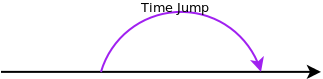
\includegraphics[scale=0.5]{./images/forward.png}

\paragraph{Grandfather Assassination Failed}
Another hypothesis of how time travel could exist is called \emph{The Timeline Protection Hypothesis} which describes a basic law of nature that states that time travel can never create a paradox. So by design, this hypothesis describes a universe where time travel can exist without a paradox. Whenever someone travels back in time a distortion of probability takes place. Because of this probability distortion all attempts to create a paradox by means of time travel will fail. For example: the time traveler's gun jammed at the moment he tried to shoot his grandfather or he accidentaly missed the shot or he didn't travel to a early enough date, so his father would have already been concieved when the grandfather was killed, etc. So the timeline protects itself by turning all odds against the time traveler that is trying to create a paradox.
\\
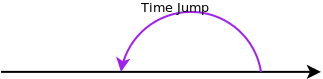
\includegraphics[scale=0.5]{./images/fail.png}

\paragraph{Im Not Your Real Grandfather}
A variant of the timeline protection hypothesis is called the Novikov self-consistency principle which also prevents these paradoxes from happening in the first place by stating that everything is predestined to happen. The time traveler that went back in time to kill his own grandfather, would for example see a man dating his grandmother and kill him assuming that this man is his grandfather. However because this man was killed the grandmother would find a new man, marry him and give birth to the time traveler's actual father. So by going back in time to kill his grandfather he actually ensured his own existance and the existance of his original future. The time traveler went back in time because he was predestined to do so. Any action that the time traveler takes will result in the same outcome. going back in time to create a paradox will always result in fullfilling his predefined destiny.
\\
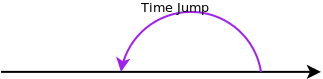
\includegraphics[scale=0.5]{./images/fail.png}
\paragraph{}
This hypothesis will eliminate the grandfather paradox, but it gives way to another one, named the bootstrap paradox. The bootrstrap paradox states that there can be no start to the cycle of future sons coming back to kill the man that is not his grandfather, and by extension allow the grandmother to remarry. Since in the first occurence there is no future son to come back, to ensure his grandmother marries his grandfather. So this destiny is not fullfilled, and that would mean that the time traveler will not be born to ensure his existance in the next iteration.\\

\paragraph{Fixpoint}
One way of mitigating this origin problem is by stating that multiple itiration of the timeline have eventually evolved into a self consistent fixpoint state where each previous itiration will ensure that the next itiration is identical. This might be because some random event caused the grandmother to remarry the time traveler's real grandfather. From that point on each future itiration of the timeline will have a time traveler going back in time to ensure his own existance as well. For each of the posible event the current timeline is in a equilibrium fixpoint state resulting in a sort of predestination feel.

\paragraph{Self Healing Timeline}
Both the timeline protection hypothesis and the Novikov Self-consistency principle might lead to some concern about free will. In both these models free will is merely an illusion or at least not boundless the way we percieve it to be. Therefore a closely related hypothesis was suggested, namely the self healing timeline hypothesis. The difference between these two hypotheses is that the time traveler can still go back in time and succeed in his apparant mission. Let's say that he was to prevent a war from happening in the future, by killing the political figure that was responsible for the start of the war. The other two models would just prevent the assasination to succeed. In the self healing timeline model he will succeed in killing the political figure. However in doing so he will upset the followers and the emotional effect would be enough to overcome the missing charisma of the killed leader. Eventually the same war will take place, the only difference will be the way it started. In short this is a more flexible approach to the predestined way of looking at the timeline. The time traveler would still not be able to create a paradox, but if he decides to do something by means of time travel, there is nothing that will, by definition, stop him from doing so.

\paragraph{Grandfather Assassination In Parallell}
Take the same example of a grandson going back in time to kill his grandfather. The moment in time where the time traveler is potentially killing his grandfather there are two options. Either the grandfather dies, or he doesn't. Both events could possibly take place. In the event that the grandfather does not die, we end up on the original timeline  where nothing has changed. If because of some series of events, for example the grandson going back in time, the grandfather ends up dying at this point a new universe is created. This new universe is parallell to the previous original universe, and up to this point the entire past will be exactly the same as the original one. But since we assume all future events to take into account all past event, the future might change. The most notable change in the future for this example is that his grandfather will not have any offspring. This means that in this instance of the universe the time traveler will not be born. But this poses no threat to the original time traveler since he was already born in another universe where a different future exists.
\\
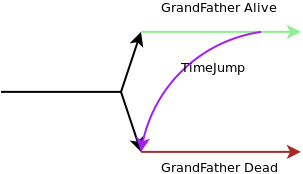
\includegraphics[scale=0.5]{./images/parallell.png}
\paragraph{}
When the time traveler decides to go back to the future he will not end up in his own universe. He would be in the future of the universe that has evolved taking into account the killling of his grandfather. Going back to the future in his own original universe will not be possible.
\paragraph{}
If the time traveler tries to go back to an even further point in time to prevent the death of his grandfather he would still not be able to go back to his original future. He would just create another parallell universe at that point. In one universe he did not succeed in preventing the death, and in the other he did succeed. It might be possible that in one of these universes his dad and granddad will be alive, and even another instance of himself is born. But this would still not be his own original future. That universe would be forever lost to him.
\\
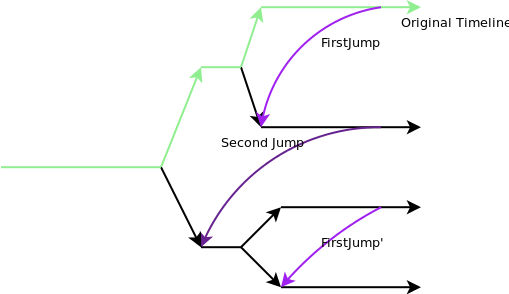
\includegraphics[scale=0.5]{./images/fixingit.png}

\paragraph{Chaos Theory}
The chaos theory describes a model in which a very small alteration of initial variables can have enormous effect in the eventual outcome. In time travel stories this effect is often called the butterfly effect. Supose a time traveler goes back in time and only change the most minor of things, for example he would just stand in a forest somewhere for a brief moment, after which he would go back to his original time. When he arives back in the future he might notice very large differences in how the history has evolved. It might be as small as a fly having to cwnavigate around him, instead of going straight, resulting in a frog eating the fly instead of the fly surviving, which would then prevent a nearby car crash of a celebrety to happen because the fly was not there to distract the driver.
Because of the complexity of the universe it is practicaly imposible to oversee all possible causal effect one might have by traveling back in time.
\paragraph{Erased Timeline}
The Erased Timeline hypothesis uses this chaos theory to overwrite the timeline  every time a change in the timeline happens. If a time traveler would go back in time to interact with the world at that time, no mather how small the change, it will always result in the entire future to be rewritten, resulting in erasing the previous original timeline. This would mean that the time traveler would never be able to go back to his own timeline either, the same as the parallell universe hypothesis. However in this model the previous timeline is completely gone, while in the parallell universe model it would still exist, it would just be unreachable. But since the time traveler is already in the current time by the time the future is erased he will have no problem with that. He would still exist, even though he has no temporal origin anymore. If we relate this to the grandfather paradox, it would not mather if the time traveler would go back to kill his grandfather. The traveler himself would come from a future that no longer exists, but he will still exist in the current time.
\paragraph{Still no Time Travelers}
Even though there are plenty of hypotheses that allow time travel to occur without causing any paradoxes we still don't have access to time travel technology. It is strange to asume that time travel technology will be invented in the future and subsequently not be brought back to a past point in time. And if the technology was made available earlier the people living in that age, one could asume that at least one of the people in that age might bring it back further to the past as well. Following this logic if the technology will be invented at any point in the future we could asume that we would have had access to time travel as early as the beginning of civilisation.
\paragraph{}
There may be a couple of scenarios why we don't have time travel technology yet. The easiest explanation is that it simply isn't possible to travel back in time, and that it never will be possible. But for all the science fiction lovers this does not seem like a acceptable explanation. A popular explanation is that time travel will be possible at some point in the future, but it will only go as far back into the past up to the creation of the time machine.
A second explanation might be that we are not developped enough as a society to create the means to travel through time. Even if a time traveler would come back to our time, he would not be able to teach us how to time travel because our current technology is not yet advanced enough. Of cource we could then ask why our future selves aren't going back in time to slowly teach the basics of what is needed for time travel. But can we really say they aren't? Some might say that at certain points in time we enter a so called \emph{golden age} for sience. Where people like Nikola Tesla, Niels Bohr or Albert Einstein make such a significant scientific breakthrough that we jump ahead in technology by decades. So maybe there are people going back in time to prepare our current society to handle the scientific knowledge that is needed to eventually be able to travel in time. Maybe it is just a slow process that is not yet finished.


\end{multicols}

\end{document}
